%%%%%%%%%%%%%%%%%%%%%%%%%%%%%%%%%%%%%%%%%%%%%%%%%%%%%%%%%%%%%%%%%%%%%%%%%%%%%%%%%%
\begin{frame}[fragile]\frametitle{}
\begin{center}
{\Large Conclusions}
\end{center}
\end{frame}

%%%%%%%%%%%%%%%%%%%%%%%%%%%%%%%%%%%%%%%%%%%%%%%%%%%%%%%%%%%
\begin{frame}[fragile]\frametitle{Summary}
    \begin{itemize}
        \item Enhances LLMs by linking them to diverse data sources
        \item Supports data ingestion from various formats and databases
        \item Offers a powerful query and retrieval interface
        \item Highly customizable with data connectors and loaders
        \item Suitable for chatbots, analytics, and data-augmented tasks
        \item Bridges LLMs with external knowledge for richer responses
    \end{itemize}
\end{frame}

%%%%%%%%%%%%%%%%%%%%%%%%%%%%%%%%%%%%%%%%%%%%%%%%%%%%%%%%%%%
\begin{frame}[fragile]\frametitle{Overview}

\begin{center}
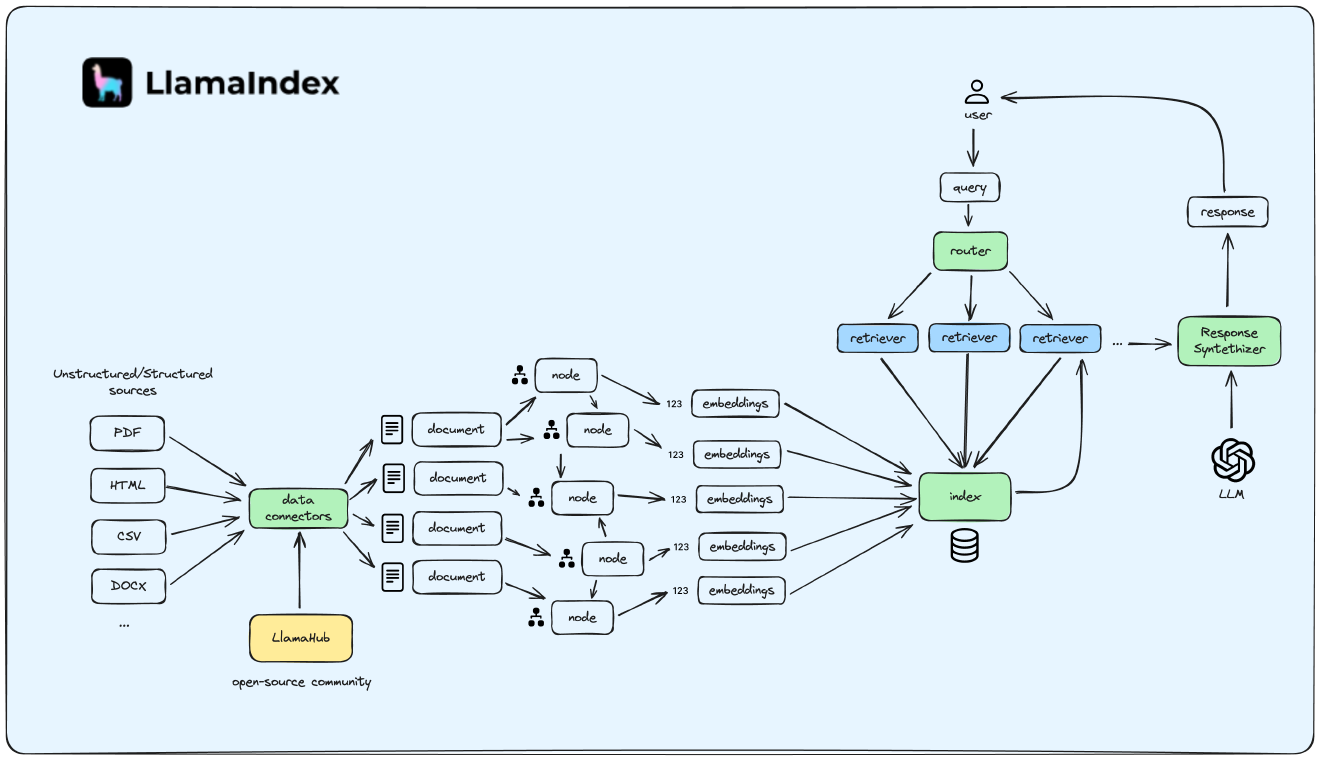
\includegraphics[width=\linewidth,keepaspectratio]{llamaindex21}

{\tiny (Ref: Introduction to LlamaIndex - Alejandro AO)}
\end{center}
\end{frame}


%%%%%%%%%%%%%%%%%%%%%%%%%%%%%%%%%%%%%%%%%%%%%%%%%%%%%%%%%%%
\begin{frame}[fragile]\frametitle{Capabilities}


\begin{itemize}
\item Handle complex queries
\item Multi-modal data management
\item Better evaluation of LLM data systems
\item Optimization of Latency/Cost
\item Ease of use for both beginner users and advanced users
\end{itemize}	

\end{frame}

%%%%%%%%%%%%%%%%%%%%%%%%%%%%%%%%%%%%%%%%%%%%%%%%%%%%%%%%%%%
\begin{frame}[fragile]\frametitle{Solving the data problem at scale for Enterprises}


\begin{itemize}
\item Production-ready data ingestion and management
\item Scale to Large Data Volumes
\item Domain-specific LLM solutions
\end{itemize}	

\end{frame}

%%%%%%%%%%%%%%%%%%%%%%%%%%%%%%%%%%%%%%%%%%%%%%%%%%%%%%%%%%%%%%%%%%%%%%%%%%%%%%%%%%
\begin{frame}[fragile]\frametitle{References}


\begin{itemize}
\item LlamaIndex: A Central Interface between LLM’s + your external data: https://github.com/jerryjliu/llama\_index
\item Llama Index and Evaluation of QA Systems - Ravi Theja

\end{itemize}


\end{frame}